%%%%%%%% ICML 2019 EXAMPLE LATEX SUBMISSION FILE %%%%%%%%%%%%%%%%%

\documentclass{article}

% Recommended, but optional, packages for figures and better typesetting:
\usepackage{microtype}
\usepackage{graphicx}
\usepackage{subfig}
\usepackage{amsmath}
\usepackage{booktabs} % for professional tables
\usepackage{caption}
\usepackage{tabu}
\usepackage{array}

\graphicspath{ {.} }

% hyperref makes hyperlinks in the resulting PDF.
% If your build breaks (sometimes temporarily if a hyperlink spans a page)
% please comment out the following usepackage line and replace
% \usepackage{icml2019} with \usepackage[nohyperref]{icml2019} above.
\usepackage{hyperref}

% Attempt to make hyperref and algorithmic work together better:
\newcommand{\theHalgorithm}{\arabic{algorithm}}

% Use the following line for the initial blind version submitted for review:
%\usepackage{icml2019}

% If accepted, instead use the following line for the camera-ready submission:
\usepackage[accepted]{icml2019}

% The \icmltitle you define below is probably too long as a header.
% Therefore, a short form for the running title is supplied here:
\icmltitlerunning{Advanced Methods in Natural Language Processing – Spring 2019}

\begin{document}

\twocolumn[
\icmltitle{Convolutional Encoder Approach to Sentence Simplification}

% It is OKAY to include author information, even for blind
% submissions: the style file will automatically remove it for you
% unless you've provided the [accepted] option to the icml2019
% package.

% List of affiliations: The first argument should be a (short)
% identifier you will use later to specify author affiliations
% Academic affiliations should list Department, University, City, Region, Country
% Industry affiliations should list Company, City, Region, Country

% You can specify symbols, otherwise they are numbered in order.
% Ideally, you should not use this facility. Affiliations will be numbered
% in order of appearance and this is the preferred way.
\icmlsetsymbol{equal}{*}

\begin{icmlauthorlist}
\icmlauthor{Yotam Manne}{equal,tau}
\icmlauthor{Guy Azov}{equal,tau}
\end{icmlauthorlist}

\icmlaffiliation{tau}{Blavatnik School of Computer Science, Tel Aviv University, Tel Aviv, Israel}

\icmlcorrespondingauthor{Yotam Manne}{yotammanne@mail.tau.ac.il}
\icmlcorrespondingauthor{Guy Azov}{guyazov@mail.tau.ac.il}

% You may provide any keywords that you
% find helpful for describing your paper; these are used to populate
% the "keywords" metadata in the PDF but will not be shown in the document
\icmlkeywords{Machine Learning, ICML}

\vskip 0.3in
]

% this must go after the closing bracket ] following \twocolumn[ ...

% This command actually creates the footnote in the first column
% listing the affiliations and the copyright notice.
% The command takes one argument, which is text to display at the start of the footnote.
% The \icmlEqualContribution command is standard text for equal contribution.
% Remove it (just {}) if you do not need this facility.

%\printAffiliationsAndNotice{}  % leave blank if no need to mention equal contribution
\printAffiliationsAndNotice{\icmlEqualContribution} % otherwise use the standard text.

\begin{abstract}
Sentence simplification aims to simplify the content and structure of complex sentences, and thus make them easier to interpret for human readers, and easier to process for downstream NLP applications. In this paper, we adapt an architecture of Encoder-Decoder model presented by \cite{DBLP:journals/corr/GehringAGD16}. Facebook's model was originally developed for Neural Machine Translation, however, we modified it for the sentence simplification task.
\end{abstract}

\section{Introduction}
\label{Intro}

The goal of sentence simplification is to convert complex sentences into simpler ones so that they are more understandable and accessible, while still keeping their original information content and meaning. Sentence simplification has a number of practical applications: it is useful for bilingual education and other language-learning contexts. It can help patients with linguistic and cognitive disabilities \cite{Carroll99simplifyingtext}. Sentence simplification can also be used to improve performance in other NLP tasks (\cite{niklaus2017sentence}; \cite{Chandrasekar:1996:MMT:993268.993361};\cite{10.1007/978-3-540-30468-5_47}.


\section{Related Work}

In previous studies, researchers of sentence-level simplification mostly address the simplification task as a machine translation problem. Specia et al. (2010) use  statistical machine translation approach implemented in Moses toolkit (Koehn et al., 2007) to translate the original sentences to the simplified ones. Wang et al. (2016) were the first to suggest using a NMT model for text simplification. They used a LSTM encoder - decoder seq2seq model, but due to the lack of an adequate dataset they used a number-based sequences instead of natural language data. Coster et al.(2011) introduced a new dataset of aligned sentence pairs taken from Wikipedia and Simple English Wikipedia, the dataset is widely used in many sentence simplification researches. Zhang et al.(2017) suggested a constrained seq2seq neural model for sentence simplification, their model combines world level and sentence level simplifications and yields better results than various baselines. Meng et al.(2015) proposed using a convolutional neural network to encode the source language for NMT. Our work is based on the model that was presented by Gehring et al.(2017) for NMT, which uses two convolutional neural networks as an encoder, and an attention based recurrent neural network as the decoder.(Flavio?)

\section{Our Approach}
We chose to adapt a NMT model to the sentence simplification task. Most of the seq2seq neural models we encountered were based on RNN encoder – decoder, however we decided to encode the source sentences with a Convolutional Neural Network instead.
\cite{DBLP:journals/corr/GehringAGD16} used a similar approach for NMT. \cite{di2019enriching} tried it too for sentence classification. But as far as we know, we are the first to try this architecture for sentence simplification.
CNNs computation, contrary to RNNs, can be parallelized, optimization is easier since the number of non-linearities is fixed and independent of the input length and last because they outperform the LSTM accuracy in \cite{DBLP:journals/corr/WuSCLNMKCGMKSJL16}.

\section{Encoder Architecture}
One of the challenges of using CNNs encoders is the loss of word ordering. In order to solve it, \cite{DBLP:journals/corr/GehringAGD16} proposes to use position embeddings in addition to the pretrained word embeddings. See table \ref{table:emb}. Let $u_j$ be the $j^{th}$ word in the source sentence, $w_j$ it's word embedding and $l_j$ it's position embedding, then:
%\vspace{5mm}
\begin{center}
$e_j = l_j + w_j$
\end{center}
%\vspace{5mm}
As suggested by \cite{DBLP:journals/corr/GehringAGD16} The encoder consists of two stacked convolutional networks: CNN-a’s output $z_{j}$ used for creating the attention matrix $A$ that is used at decoding time. Simultaneously, CNN-c’s output $z^{\prime}_{j}$ is used to produce the conditional input $c_i$ by a simple dot product between the attention vector $a_i$ with it.
\vspace{5mm}
\begin{center}
$z_j = CNN_a(\textbf{e})_j,\;z^{\prime}_{j} = CNN_c(\textbf{e})_j$
\vspace{5mm}
\end{center}

The CNNs do not contain pooling layers which are commonly used for down-sampling, i.e., the full source sequence length will be retained after the networks has been applied. Figure \ref{fig:enc} visualizes the encoder architecture.


\begin{center}
\begin{table}[h]
 \begin{tabu}  { | X[0.8,l] | X[0.8,l] | X[3,l] | }
 \hline
 Word & Position & Representation \\
 \hline
 we & 1 & WordEmbedding(we) +\linebreak PositionEmbedding(1)  \\ 
 \hline
 need & 2 & WordEmbedding(need) +\linebreak PositionEmbedding(2)\\
 \hline
  a & 3 & WordEmbedding(a) +\linebreak PositionEmbedding(3)\\
 \hline
 vacation & 4 & WordEmbedding(vacation) +\linebreak PositionEmbedding(4)\\
 \hline
\end{tabu}
\caption{Embedding of a full sentence}
\label{table:emb}
\end{table}
\end{center}

\begin{figure}[h]
    \centering
	\captionsetup{justification=centering,margin=2cm}
    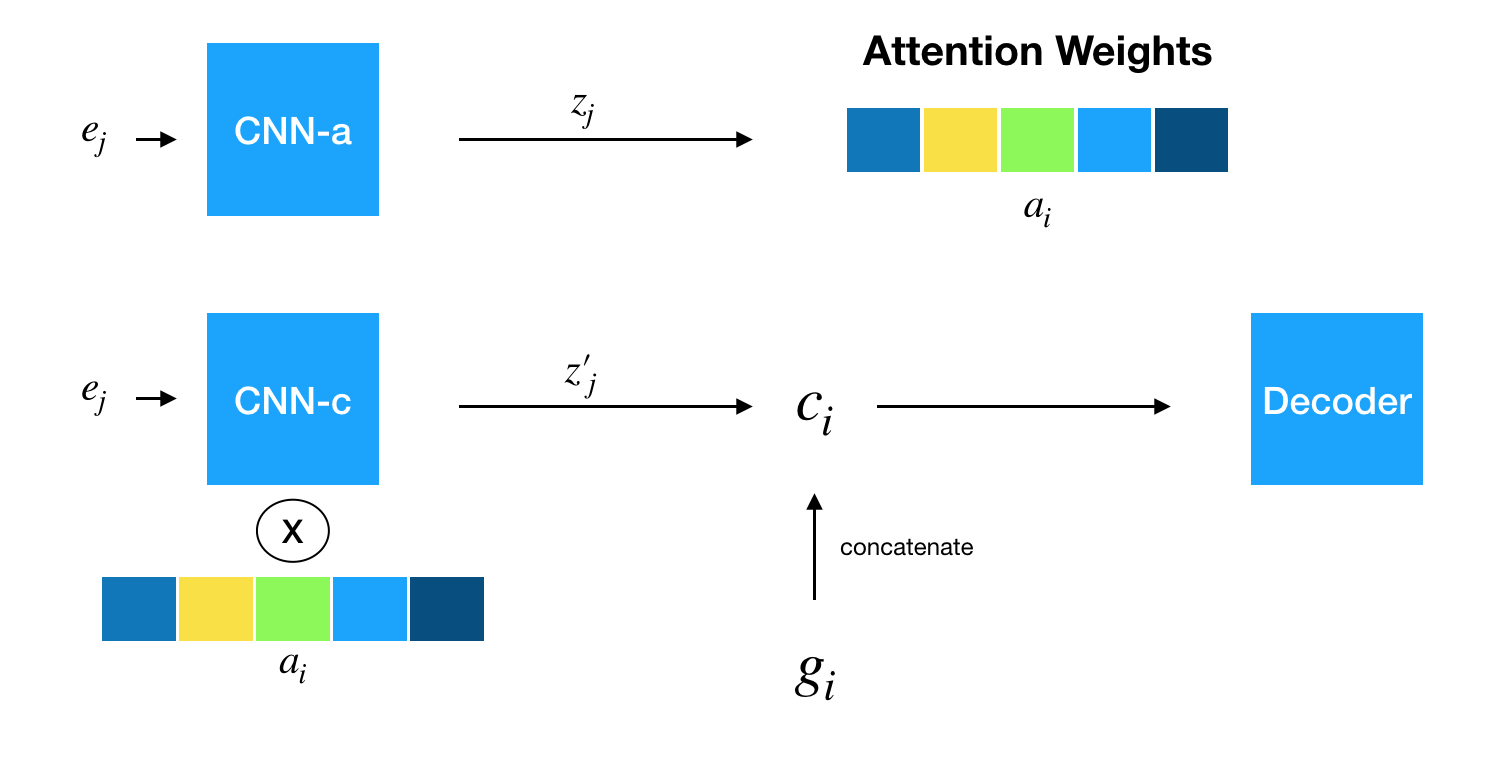
\includegraphics[scale=0.35]{Encoder_Flow}
    \caption{Block diagram of the Encoder flow and architecture}
    \label{fig:enc}
\end{figure}

\section{Decoder Architecture}
\subsection{Preliminaries}
\begin{itemize}
\item $h_i$ denotes the hidden state/output of the LSTM.
\item $c_i$ denotes the conditional input to the LSTM.
\item $g_i$ denotes the embedding of the previous output of the LSTM. This gets concatenated with $c_i$ as input to the LSTM
\end{itemize}

\begin{flushleft}

\subsection{Attention}
At time step $i$ the conditional inpul $c_i$ is computed via a dot product attention mechanism \cite{luong2015effective}. We transform the decoder hidden state $h_i$ by a linear layer with weights $W_d$ and $b_d$ to match the size of the embedding of the previous target word $g_i$ and then sum the two representations to yield $d_i$:
\begin{center}
$d_i=W_dh_{i}+b_d+g_i$
\end{center}
Next, we generate the attention matrix $A$ as follows:
$$a_{ij} = \frac{exp \left(d_i^Tz_j\right)}{\sum^m_{t=1}exp\left(d_i^Tz_t\right)}$$
Instead of generating $a_{ij}$ individually, we can generate the entire $\mathbf{a_i}$ in one go, by modifying the equation slightly:
$$\mathbf{a_i} = \text{softmax}(d_i^T\mathbf{z})$$
Finally, we generate $c_i$ as:\linebreak
$c_i = \sum_{j=1}^{m}a_{ij}z^{\prime}_{j}$

\begin{figure}[h]
    \centering
	\captionsetup{justification=centering,margin=2cm}
    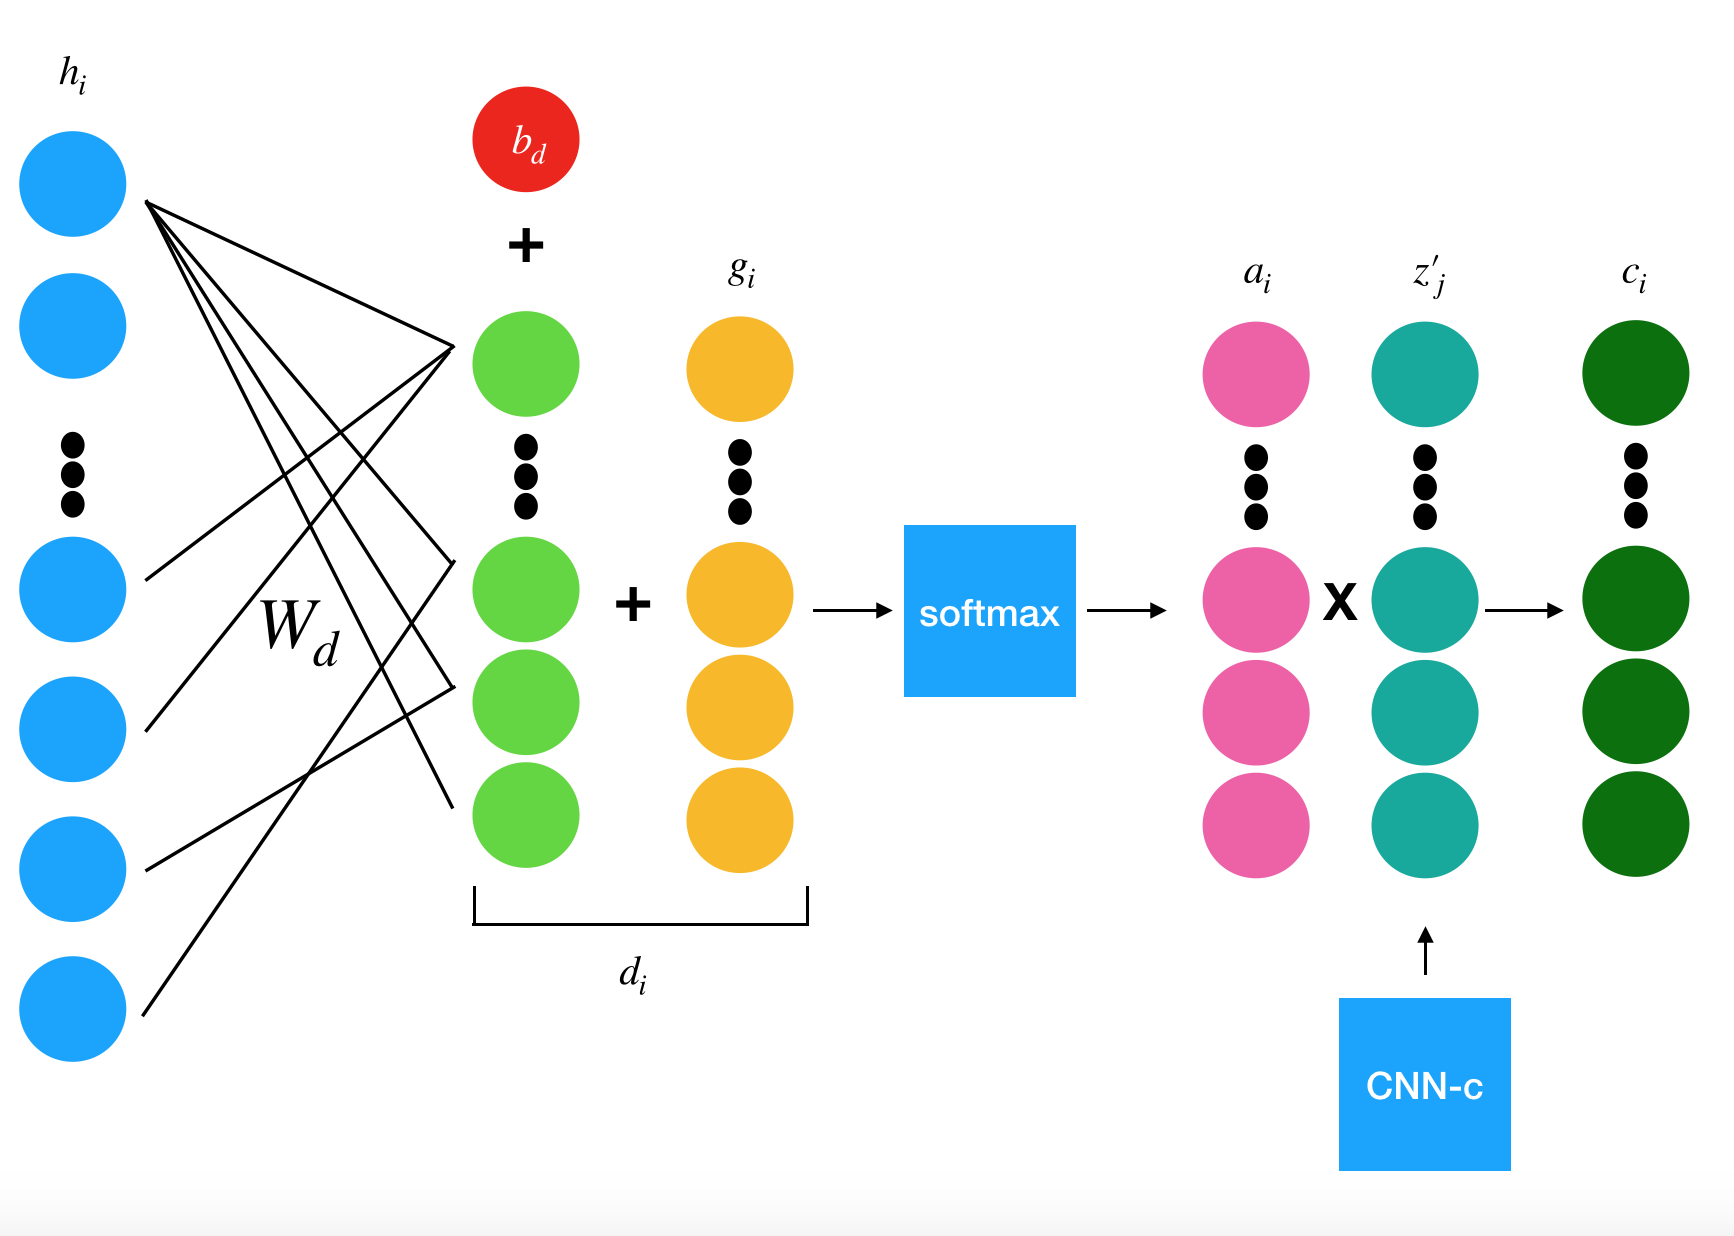
\includegraphics[scale=0.25]{Attention}
    \caption{The dot product attention mechanism}
    \label{fig:att}
\end{figure}

\subsection{The Decoder}
We use LSTMs \cite{hochreiter1997lstm} for the decoder network whose state $s_i$ comprises of a cell vector and a hidden vector $h_i$ which is output by the LSTM at each time step. We concatenate $c_i$ and $g_i$, and feed them into the LSTM .
The decoder output $h_{i+1}$ is transfromed by a linear layer with weights $W_o$ and bias $b_o$ to the target vocabulary size $V$, then a softmax layer is applied to create a distribution over all possible words. The most probable word will be selected as the decoder's output $y_{i+1}$. 
\vspace{5mm}
\begin{center}
$y_{i+1}=argmax(softmax(W_oh_{i+1}+b_o))$\vspace{5mm}
\end{center}

\end{flushleft}

\begin{figure}[h]
    \centering
	\captionsetup{justification=centering,margin=2cm}
    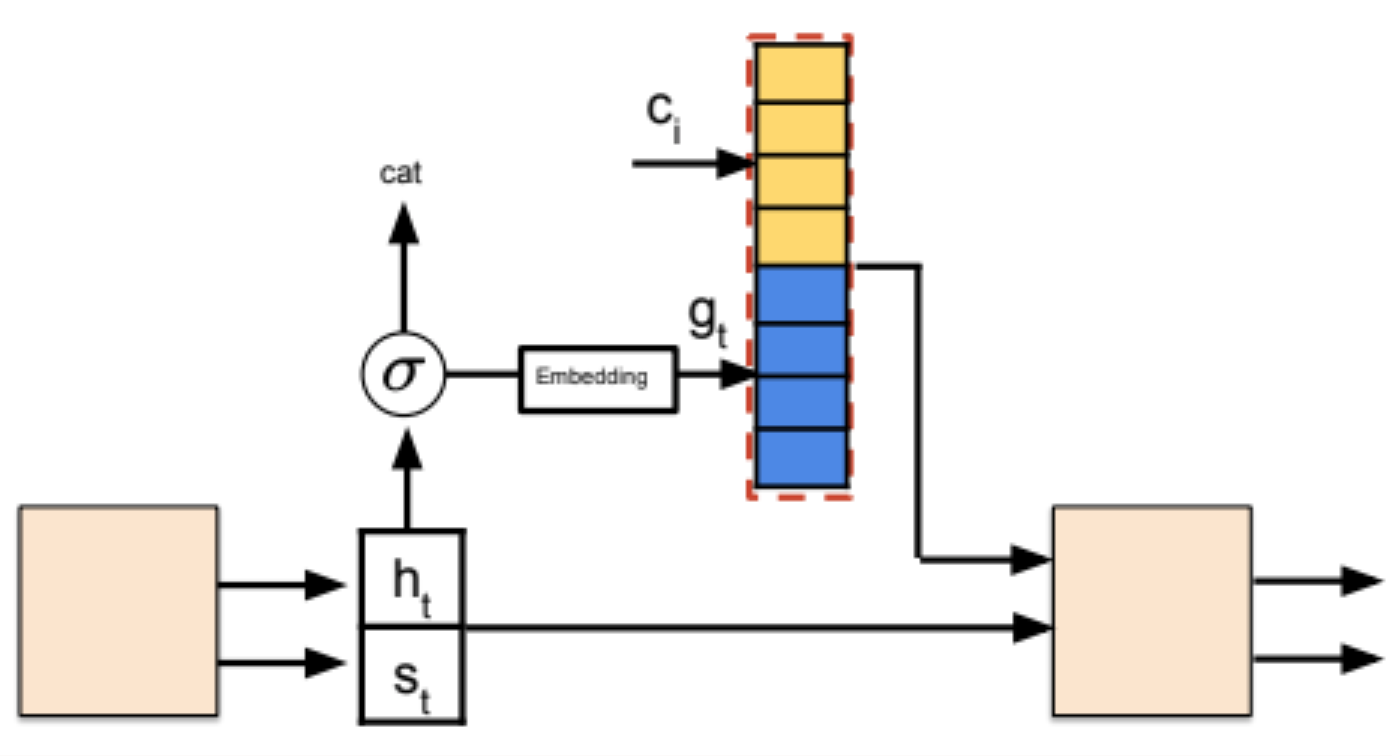
\includegraphics[scale=0.35]{Decoder_Flow}
    \caption{Block diagram of the Decoder flow and architecture}
    \label{fig:dec}
\end{figure}

\section{Experimental Setup}
\subsection{Datasets}

\subsubsection{Simple English Wikipedia \cite{coster-kauchak-2011-simple}}
A sentence aligned dataset taken from parallel articles in English Wikipedia and Simple English Wikipedia. This dataset contains 167K pairs of sentences and is one of the largest datasets used for sentence simplification. While examining this dataset we noticed a few problems – Many sentences contain special characters, URLs, gibberish, excess use of punctuation and more. <example>. Such anomalies can interfere the training procedure and cause unreliable results.

\subsubsection{Newsela \cite{Xu-EtAl:2015:TACL}}
A simplification corpus of news articles, re-written by professional editors to meet the readability standards for children at multiple grade levels. Each sentence in the corpus is rewritten in up to 6 different level of complexity. The creators of this dataset mapped all the problems that exist in the Simple Wikipedia corpus and addressed them in their research. The Newsela dataset contains 141K pairs of aligned sentences.
Our model supports both datasets but because of the problems we mentioned above we used the Newsela corpus for training and evaluation.


\subsection{Data Preprocessing}
To use the data we needed some pre-processing. Two aligned lists of sentences were constructed from the raw data. From each list a vocabulary which maps each word to a unique integer ID was created. Using the mentioned vocabularies, every sentence was converted to a list of word IDs. Each tokenized sentence is fed later as input to our model, which uses GloVe embeddings \cite{pennington2014glove} to represent each word in lower dimensional space.

\subsection{Control}
results of classic encoder - decoder model.

\subsection{Model Benchmarking}
Overfit our model for sanity check
Run on full dataset (describe parameters used)

\subsection{Optimization}
	Parameters tuning \cite{neishi2017bag}
	Teacher forcing
	Custom loss?
	Weighted sum instead of argmax (cite jonathan)

\section{Future Work}
	Loss?
	Beam search
	Optimize code for parallelism (multiple GPUs etc)
	More epochs maybe on faster system


%\begin{algorithm}[tb]
%   \caption{Bubble Sort}
%   \label{alg:example}
%\begin{algorithmic}
%   \STATE {\bfseries Input:} data $x_i$, size $m$
%   \REPEAT
%   \STATE Initialize $noChange = true$.
%   \FOR{$i=1$ {\bfseries to} $m-1$}
%   \IF{$x_i > x_{i+1}$}
%   \STATE Swap $x_i$ and $x_{i+1}$
%   \STATE $noChange = false$
%   \ENDIF
%   \ENDFOR
%   \UNTIL{$noChange$ is $true$}
%\end{algorithmic}
%\end{algorithm}

\nocite{*}
\bibliography{example_paper}
\bibliographystyle{icml2019}



\end{document}


% This document was modified from the file originally made available by
% Pat Langley and Andrea Danyluk for ICML-2K. This version was created
% by Iain Murray in 2018, and modified by Alexandre Bouchard in
% 2019. Previous contributors include Dan Roy, Lise Getoor and Tobias
% Scheffer, which was slightly modified from the 2010 version by
% Thorsten Joachims & Johannes Fuernkranz, slightly modified from the
% 2009 version by Kiri Wagstaff and Sam Roweis's 2008 version, which is
% slightly modified from Prasad Tadepalli's 2007 version which is a
% lightly changed version of the previous year's version by Andrew
% Moore, which was in turn edited from those of Kristian Kersting and
% Codrina Lauth. Alex Smola contributed to the algorithmic style files.
